\subsection{Modello del sensore ed Occupacy grid}

Gli approcci basati sulle occupacy grid tendono a non ragionare sulla geometria delle caratteristiche  dell'ambiente, ma ad assumere una visione più sensoriale. Una rete di celle (una griglia) è posta sopra il
(inizialmente sconosciuto) mondo. Ogni cella c (i; j) ha un numero associato ad essa corrispondente
a una probabilità di occupazione - po (i; j) e una probabilità di essere vuoto pe. Non facciamo affermazioni in merito ciò che sta occupando solo che qualcosa o parte di qualcosa è alle coordinate coperte
per cella (40,20).

\subsubsection{Occupacy grid locale}
Per un determinato sensore di rilevamento della distanza, come uno scanner per linee laser, con portata massima R e mezza larghezza del raggio del sensore $\beta$, il modello può essere scomposto in un numero di settori etichettati I-IV, come illustrato nella Figura. .

\begin{figure}
  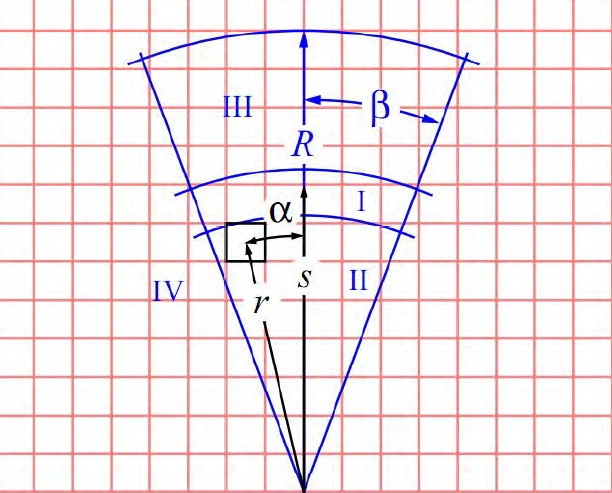
\includegraphics[scale = 0.35]{occ_grid_model.jpeg}
  \caption{Scan scheme}
  \label{fig:scan scheme}
\end{figure}

La regione I è la regione associata alla lettura effettiva del laser, la regione II rappresenta un'area vuota in cui nulla viene rilevato,la regione III è l'area coperta dal raggio laser, ma rimane sconosciuto se è occupata o meno a causa dell'occlusione,e la regione IV è al di fuori del campo di visibilità del Lidar.

Parametri rilevanti per il ragionamento sulla cella evidenziata (contorno nero) includere r, che è la distanza dell'elemento di griglia dalla posizione del sensore, e $\alpha$, l'angolo dell'elemento di griglia relativo al raggio centrale del sensore.

Per una misurazione s che ricade nella regione I, la probabilità che la misura fosse dovuta a un
ostacolo effettivo presente a tale intervallo e il suo complemento può essere calcolato da:

\begin{equation}	
\label{eq:lidargrid}
P(s|Occupied) = \frac{\frac{R-r}{R} + \frac{ \beta- \alpha}{\beta} \beta}{2}*Max_{occupied}
\end{equation}

dove Maxoccupato è dovuto all'assunzione che una lettura di "Occupato" non è mai completamente
affidabile.
A causa dell'occlusione, assumiamo che la probabilità di occupazione nella regione III sia del 50%
occupato e il 50 $\%$ non occupato.

\subsubsection{Occupacy grid globale}
Ogni robot presenta al suo interno un memoria interna che tiene conto di una possibile mappatura globale dell'intero ambiente. Questa è definita occupacy grid globale e viene ricostruita rototraslando le varie occupacy grid locali fornite in diversi istanti dal robot.

Un problema con i metodi basati sulla griglia è l'utilizzo della memoria: diventa costoso per il 3D
mappe. Un secondo problema è quello della griglia allineamento - è arbitrario e in quanto tale è probabile che le celle coprano aree che sono difficili da raggiungere parzialmente pieno come tale non è possibile catturare le acute discontinuità ai bordi di oggetti. Forse il più grande problema dei metodi basati sulla griglia deriva dalle difficoltà in localizzazione rispetto a una griglia.